\documentclass[tikz]{standalone}
\usepackage{tikz,pgffor}
\usetikzlibrary{arrows,decorations.pathmorphing, backgrounds, positioning, fit, petri}
\tikzset{ 
	seagull/.pic ={
		\draw (-3mm,0) to [bend left] (0,0) to [bend left] (3mm,0);
	}
}


\begin{document}
	  
	\pgfdeclarelayer{bg}
	\pgfdeclarelayer{fg}
	\pgfsetlayers{bg,main,fg}
 			
			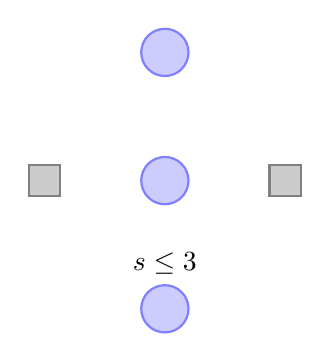
\begin{tikzpicture}
				[ 
				place/.style={circle, draw=blue!50, fill=blue!20, thick, minimum size=6mm}, 
				transition/.style={rectangle,draw=black!50, fill=black!20, thick, minimum size=4mm}]
				\node [place]  			(waiting 1)			 					 					{} ;
				\node [place]  			(critical 1)			[below= of waiting 1]		{}; 
				\node [place] 			(semphore)			[below=of critical 1, label=above:$s\le3$] 		{};
				\node [transition]  	(leave critical)	[right=of critical 1]{} ;
				\node [transition] 		(enter critical) 	 [left=of critical 1]{};
			\end{tikzpicture}		
		
\end{document}